\documentclass[../main.tex]{subfiles}






\begin{document}
\chapter{}
\label{cha:cha_20}

\section{}
The matrix inverse can be evaluated and the power method expressed as
	\bigbreak
$
\left[\begin{array}{ccc}
0.0375 & 0.025 & 0.0125 \\
0.025 & 0.05 & 0.025 \\
0.0125 & 0.025 & 0.0375
\end{array}\right]-\lambda[I]=0
$
	\bigbreak
Iteration 1:
	\bigbreak
$
\left[\begin{array}{ccc}
0.0375 & 0.025 & 0.0125 \\
0.025 & 0.05 & 0.025 \\
0.0125 & 0.025 & 0.0375
\end{array}\right]\left\{\begin{array}{l}
1 \\
1 \\
1
\end{array}\right\}=\left\{\begin{array}{c}
0.075 \\
0.1 \\
0.075
\end{array}\right\}=0.1\left\{\begin{array}{c}
0.75 \\
1 \\
0.75
\end{array}\right\}
$
	\bigbreak
Iteration 2:
	\bigbreak
$
\left[\begin{array}{ccc}
0.0375 & 0.025 & 0.0125 \\
0.025 & 0.05 & 0.025 \\
0.0125 & 0.025 & 0.0375
\end{array}\right]\left\{\begin{array}{c}
0.75 \\
1 \\
0.75
\end{array}\right\}=\left\{\begin{array}{c}
0.0625 \\
0.0875 \\
0.0625
\end{array}\right\}=0.0875\left\{\begin{array}{c}
0.71428571 \\
1 \\
0.71428571
\end{array}\right\}
$
	\bigbreak
$\varepsilon_{a}=\left|\dfrac{0.0875-0.1}{0.0875}\right| \times 100 \%=14.29 \%$
	\bigbreak
Iteration 3:
	\bigbreak
$
\left[\begin{array}{ccc}
0.0375 & 0.025 & 0.0125 \\
0.025 & 0.05 & 0.025 \\
0.0125 & 0.025 & 0.0375
\end{array}\right]\left\{\begin{array}{c}
0.71428571 \\
1 \\
0.71428571
\end{array}\right\}=\left\{\begin{array}{c}
0.060714 \\
0.085714 \\
0.060714
\end{array}\right\}=0.085714\left\{\begin{array}{l}
0.708333 \\
1 \\
0.708333
\end{array}\right\}
$
	\bigbreak
$\varepsilon_{a}=\left|\dfrac{0.085714-0.0875}{0.085714}\right| \times 100 \%=2.08 \%$
	\bigbreak
The iterations can be continued. After 10 iterations, the relative error falls to $0.00000884 \%$ with the result
	\bigbreak
$
0.085355\left\{\begin{array}{c}
0.70710678 \\
1 \\
0.70710678
\end{array}\right\}
$
	\bigbreak
Thus, the smallest eigenvalue is $1 / 0.085355=11.71573$.
	\bigbreak



\section{} \label{sec:sec_20_2}
\begin{enumerate}[label=\bfseries(\alph*)]
\item Minors:
	\bigbreak
$
(2-\lambda)\left|\begin{array}{cc}
3-\lambda & 4 \\
4 & 7-\lambda
\end{array}\right|-2\left|\begin{array}{cc}
8 & 4 \\
10 & 7-\lambda
\end{array}\right|+10\left|\begin{array}{cc}
8 & 3-\lambda \\
10 & 4
\end{array}\right|=-\lambda^{3}+10 \lambda^{2}+101 \lambda+18
$ \label{equ:equ_20_1}
	\bigbreak
\item The eigenvalues can be determined by finding the roots of the characteristic polynomial determined in \ref{equ:equ_20_1}. This can be done in MATLAB,
	\bigbreak
\begin{lstlisting}[numbers=none]
>> a = [1.0000 -10.0000 -101.0000 -18.0000];
>> roots(a)


ans =
	 16.2741
	 -6.0926
	 -0.1815
\end{lstlisting}
	\bigbreak
\item 
	\bigbreak
The power method for the highest eigenvalue can be implemented with MATLAB commands,
	\bigbreak
\begin{lstlisting}[numbers=none]
>> A = [2 2 10;8 3 4;10 4 5];
>> x = [1 1 1]'; 
\end{lstlisting}
	\bigbreak
First iteration:
	\bigbreak
\begin{lstlisting}[numbers=none]
>> x = A*x
x =
	 14
	 15
	 19


>> e = max(x)
e =


	 19
>> x = x/e
x =
	 0.7368
	 0.7895
	 1.0000
\end{lstlisting}
	\bigbreak
Second iteration:
	\bigbreak
\begin{lstlisting}[numbers=none]
>> x = A*x
x =
	 13.0526
	 12.2632
	 15.5263


>> e = max(x)
e =
	 15.5263


>> x = x/e
x =
	 0.8407
	 0.7898
	 1.0000 
\end{lstlisting}
	\bigbreak
Third iteration:
	\bigbreak
\begin{lstlisting}[numbers=none]
>> x = A*x
x =
	 13.2610
	 13.0949
	 16.5661


>> e = max(x)
e =
	 16.5661


>> x = x/e
x =
	 0.8005
	 0.7905
	 1.0000 
\end{lstlisting}
	\bigbreak
Fourth iteration:
	\bigbreak
\begin{lstlisting}[numbers=none]
>> x = A*x
x =
	 13.1819
	 12.7753
	 16.1668


>> e = max(x)
e =
	 16.1668


>> x = x/e
x =
	 0.8154
	 0.7902
	 1.0000 
\end{lstlisting}
	\bigbreak
\begin{blockquote}
Thus, after four iterations, the result is converging on a highest eigenvalue of 16.2741 with
a corresponding eigenvector of [0.811 0.790 1]. 
\end{blockquote}
	\bigbreak
\item The power method for the lowest eigenvalue can be implemented with MATLAB commands,
	\bigbreak
\begin{lstlisting}[numbers=none]
>> A = [2 2 10;8 3 4;10 4 5];
>> x = [1 1 1]';
>> AI = inv(A)


AI =
	 -0.0556	 1.6667	 -1.2222
	 -0.0000	 -5.0000	 4.0000
	 0.1111	 0.6667	 -0.5556 
\end{lstlisting}
	\bigbreak
First iteration:
	\bigbreak
\begin{lstlisting}[numbers=none]
>> x = AI*x
x =
	 0.3889
	 -1.0000
	 0.2222


>> [e,i] = max(abs(x))
e =
	 1
i =
	 2


>> x = x/x(i)
x =
	 -0.3889
	 1.0000
	 -0.2222 
\end{lstlisting}
	\bigbreak
Second iteration:
	\bigbreak
\begin{lstlisting}[numbers=none]
>> x = AI*x
x =
	 1.9599
	 -5.8889
	 0.7469


>> [e,i] = max(abs(x))
e =
	 5.8889
i =
	 2


>> x = x/x(i)
x =
	 -0.3328
	 1.0000
	 -0.1268 
\end{lstlisting}
	\bigbreak
Third iteration:
	\bigbreak
\begin{lstlisting}[numbers=none]
>> x = AI*x
x =
	 1.8402
	 -5.5073
	 0.7002


>> [e,i] = max(abs(x))
e =
	 5.5073
i =
	 2


>> x = x/x(i)
x =
	 -0.3341
	 1.0000
	 -0.1271
\end{lstlisting}
	\bigbreak
Thus, after three iterations, the estimate of the lowest eigenvalue is converging on the correct value of $1 /(-5.5085)=-0.1815$ with an eigenvector of $[-0.33411-0.1271]$.
	\bigbreak
\end{enumerate}



\section{}
\begin{blockquote}
MATLAB can be used to solve for the eigenvalues with the polynomial method. First, the matrix can be put into the proper form for an eigenvalue analysis by bringing all terms to the left-hand-side of the equation.
\end{blockquote}
	\bigbreak
$\left[\begin{array}{ccc}4-9 \lambda & 7 & 3 \\
 7 & 8-4 \lambda & 2 \\
 3 & 2 & 1-2 \lambda\end{array}\right]\left\{\begin{array}{l}x_{1} \\ x_{2} \\ 
x_{3}\end{array}\right\}=0$
	\bigbreak
Then, each row can be divided by the coefficient of $\lambda$ in that row.
	\bigbreak
$\left[\begin{array}{ccc}0.4444-\lambda & 0.7778 & 0.3333 \\
 1.75 & 2-\lambda & 0.5 \\
 1.5 & 1 & 0.5-\lambda\end{array}\right]\left\{\begin{array}{l}x_{1} \\ x_{2} \\
 x_{3}\end{array}\right\}=0$
	\bigbreak
MATLAB can then be used to determine the eigenvalues as the roots of the characteristic polynomial,
	\bigbreak
\begin{lstlisting}[numbers=none]
>> A=[4/9 7/9 3/9;7/4 8/4 2/4;3/2 2/2 1/2];
>> p=poly(A)
p =
	 1.0000	 -2.9444	 -0.2500	 0.2917


>> e=roots(p)
e =
	 2.9954
	 -0.3386
	 0.2876 
\end{lstlisting}
	\bigbreak



\section{}
\begin{enumerate}[label=\bfseries(\alph*)]
\item MATLAB can be used to solve for the eigenvalues with the polynomial method. First, the matrix can be put into the proper form by dividing each row by $0.36$.
	\bigbreak
\begin{lstlisting}[numbers=none]
>> A = [2/.36 -1/.36 0 0;-1/.36 2/.36 -1/.36 0;0 -1/.36 2/.36 -
1/.36;0 0 -1/.36 2/.36]


A =
	 5.5556	 -2.7778	  0	 	 0
	 -2.7778	 5.5556	 -2.7778	 0
	 0 		-2.7778	  5.5556	-2.7778
	 0		 0	 	 -2.7778 	5.5556 
\end{lstlisting}
	\bigbreak
Then, the poly function can be used to generate the characteristic polynomial,
	\bigbreak
\begin{lstlisting}[numbers=none]
>> p = poly(A)
p =
	 1.0000	 -22.2222	 162.0370	 -428.6694	 297.6871
\end{lstlisting}
	\bigbreak
The roots of this equation represent the eigenvalues,
	\bigbreak
\begin{lstlisting}[numbers=none]
>> e = roots(p)
e =
	 10.0501
	 7.2723
	 3.8388
	 1.0610
\end{lstlisting}
	\bigbreak
\item The power method can be used to determine the highest eigenvalue:
	\bigbreak
\begin{lstlisting}[numbers=none]
>> A = [2/.36 -1/.36 0 0;
-1/.36 2/.36 -1/.36 0;
0 -1/.36 2/.36 -1/.36;
0 0 -1/.36 2/.36];
>> x = [1 1 1 1]'; 
\end{lstlisting}
	\bigbreak
First iteration:
	\bigbreak
\begin{lstlisting}[numbers=none]
>> x = A*x
x = 
	 2.7778
		 0
		 0
	 2.7778
>> e = max(x)
e =
	 2.7778
>> x = x/e
	x =
	 1
	 0
	 0
	 1
\end{lstlisting}
	\bigbreak
Second iteration:
	\bigbreak
\begin{lstlisting}[numbers=none]
>> x = A*x
x =
	 5.5556
	 -2.7778
	 -2.7778
	 5.5556
>> e = max(x)
e =
	 5.5556
>> x = x/e
x =
	 1.0000
	 -0.5000
	 -0.5000
	 1.0000 
\end{lstlisting}
	\bigbreak
Third iteration:
	\bigbreak
>> x = A*x
x =
	 6.9444
	 -4.1667
	 -4.1667
	 6.9444
>> e = max(x)
e =
	 6.9444
>> x = x/e
x =
	 1.0000
	 -0.6000
	 -0.6000
	 1.0000
	\bigbreak
The process can be continued. After 9 iterations, the method does not converge on the highest eigenvalue. Rather, it converges on the second highest eigenvalue of $7.2723$ with a corresponding eigenvector of $[1-0.6180-0.61801]$.
	\bigbreak
\item The power method can be used to determine the lowest eigenvalue by first determining the matrix inverse:
	\bigbreak
\begin{lstlisting}[numbers=none]
>> A = [2/.36 -1/.36 0 0;-1/.36 2/.36 -1/.36 0;0 -1/.36 2/.36 -
1/.36;0 0 -1/.36 2/.36];
>> AI = inv(A)
AI =
	 0.2880	 0.2160	 0.1440	 0.0720
	 0.2160	 0.4320	 0.2880	 0.1440
	 0.1440	 0.2880	 0.4320	 0.2160
	 0.0720	 0.1440	 0.2160	 0.2880
>> x = [1 1 1 1]'; 
\end{lstlisting}
	\bigbreak
First iteration:
	\bigbreak
\begin{lstlisting}[numbers=none]
>> x = AI*x
x =
	 0.7200
	 1.0800
	 1.0800
	 0.7200
>> e = max(x)
e =
	 1.0800
>> x = x/e
x =
	 0.6667
	 1.0000
	 1.0000
	 0.6667 
\end{lstlisting}
	\bigbreak
Second iteration:
	\bigbreak
\begin{lstlisting}[numbers=none]
>> x = AI*x
x =
	 0.6000
	 0.9600
	 0.9600
	 0.6000
>> e = max(x)
e =
	 0.9600
>> x = x/e
x =
	 0.6250
	 1.0000
	 1.0000
	 0.6250
\end{lstlisting}
	\bigbreak
Third iteration:
	\bigbreak
\begin{lstlisting}[numbers=none]
>> x = AI*x
x =
	 0.5850
	 0.9450
	 0.9450
	 0.5850
>> e = max(x)
e =
	 0.9450
>> x = x/e
x =
	 0.6190
	 1.0000
	 1.0000
	 0.6190 
\end{lstlisting}
	\bigbreak
The process can be continued. After 9 iterations, the method converges on the lowest eigenvalue of $1 / 0.9450=1.0610$ with a corresponding eigenvector of [0.6180  1 1 0.6180].
	\bigbreak
\end{enumerate}



\section{}
The parameters can be substituted into force balance equations to give
	\bigbreak
$
\begin{array}{c}
\left(0.45-\omega^{2}\right) X_{1} \quad-0.2 \quad X_{2} \quad=0\\
-0.24 \quad X_{1}+\left(0.42-\omega^{2}\right) X_{2},-0.18 \quad X_{3}=0\\
-0.225 \quad X_{2}+\left(0.225-\omega^{2}\right) X_{3}=0
\end{array}
$
	\bigbreak
A MATLAB session can be conducted to evaluate the eigenvalues and eigenvectors as
	\bigbreak
\begin{lstlisting}[numbers=none]
>> A = [0.450 -0.200 0.000;-0.240 0.420 -0.180;0.000 -0.225 0.225];
>> [v,d] = eig(A)
v =
	 -0.5879	 -0.6344 	0.2913
	 0.7307	 -0.3506 	0.5725
	 -0.3471	 0.6890 	0.7664
d =
	 0.6986 	0 		0
	 0 		0.3395 	0
	 0 		0 		0.0569
\end{lstlisting}
	\bigbreak
\begin{blockquote}
Therefore, the eigenvalues are $0.6986,0.3395$ and $0.0569$. The corresponding eigenvectors are (normalizing so that the amplitude for the third floor is one),
\end{blockquote}
	\bigbreak
$
\left\{\begin{array}{c}
1.693748 \\
-2.10516 \\
1
\end{array}\right\} \quad\left\{\begin{array}{c}
-0.92075 \\
-0.50885 \\
1
\end{array}\right\} \quad\left\{\begin{array}{c}
0.380089 \\
0.746999 \\
1
\end{array}\right\}
$
	\bigbreak
A graph can be made showing the three modes
	\bigbreak
	\begin{figure}[H]
		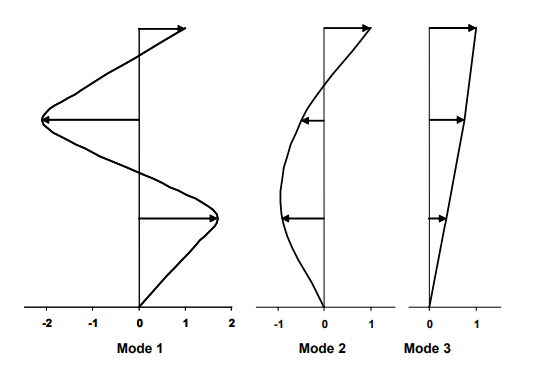
\includegraphics[width=0.5\linewidth]{fig_20_1}
		\label{fig:fig_20_1}
	\end{figure}
	\bigbreak



\section{}
As was done in Section 20.2, assume that the solution is $i_{j}=I_{j} \sin (\omega t)$. Therefore, the second derivative is
	\bigbreak
$\dfrac{d^{2} i_{j}}{d t^{2}}=-\omega^{2} I_{j} \sin (\omega t)$
	\bigbreak
Substituting these relationships into the differential equations gives
	\bigbreak
$-L_{1} \omega^{2} I_{1} \sin (\omega t)+\dfrac{1}{C_{1}}\left(I_{1} \sin (\omega t)-I_{2} \sin (\omega t)\right)=0$
	\bigbreak
$-L_{2} \omega^{2} I_{2} \sin (\omega t)+\dfrac{1}{0.001}\left(I_{2} \sin (\omega t)-I_{3} \sin (\omega t)\right)-\dfrac{1}{0.001}\left(I_{1} \sin (\omega t)-I_{2} \sin (\omega t)\right)=0$
	\bigbreak
$-L_{3} \omega^{2} I_{3} \sin (\omega t)+\dfrac{1}{0.001} i_{3}-\dfrac{1}{0.001}\left(I_{2} \sin (\omega t)-I_{3} \sin (\omega t)\right)=0$
	\bigbreak
All the $\sin (\omega t)$ terms can be cancelled. In addition, the $L$ 's and $C$ 's are constant. Therefore, the system simplifies to
	\bigbreak
$
\left[\begin{array}{ccc}
1-\lambda & -1 & 0 \\
-1 & 2-\lambda & -1 \\
0 & -1 & 2-\lambda
\end{array}\right]\left\{\begin{array}{l}
I_{1} \\
I_{2} \\
I_{3}
\end{array}\right\}=0
$
	\bigbreak
where $\lambda=L C \omega^{2}$. The following MATLAB session can then be used to evaluate the eigenvalues and eigenvectors
	\bigbreak
\begin{lstlisting}[numbers=none]
>> a = [1 -1 0;-1 2 -1;0 -1 2]
>> [v,d] = eig(a)
v =
	 -0.7370	 -0.5910	 0.3280
	 -0.5910	 0.3280	 -0.7370
	 -0.3280	 0.7370	 0.5910
d =
 	0.1981	 0	 	0
	 0 		1.5550 	0
	 0 		0 		3.2470
\end{lstlisting}
	\bigbreak
\begin{blockquote}
The matrix $v$ consists of the system's three eigenvectors (arranged as columns), and $d$ is a matrix with the corresponding eigenvalues on the diagonal. Thus, MATLAB computes that the eigenvalues are $\lambda=0.1981,1.5550$, and $3.2470$. These values in turn can be used to compute the natural frequencies for the system
\end{blockquote}
	\bigbreak
$
\omega=\left\{\begin{array}{c}
\dfrac{0.4450}{\sqrt{L C}} \\
\dfrac{1.2470}{\sqrt{L C}} \\
\dfrac{1.8019}{\sqrt{L C}}
\end{array}\right\}
$
	\bigbreak



\section{}
The force balances can be written as
	\bigbreak
$
\left[\begin{array}{ccc}
m_{1} & 0 & 0 \\
0 & m_{2} & 0 \\
0 & 0 & m_{3}
\end{array}\right]\left\{\begin{array}{l}
\ddot{x}_{1} \\
\ddot{x}_{2} \\
\ddot{x}_{3}
\end{array}\right\}+\left[\begin{array}{ccc}
2 k & -k & -k \\
-k & 2 k & -k \\
-k & -k & 2 k
\end{array}\right]\left\{\begin{array}{l}
x_{1} \\
x_{2} \\
x_{3}
\end{array}\right\}=0
$
	\bigbreak
Assuming that the solution is $x_{i}=X_{i} \sin (\omega t)$, we get the following matrix
	\bigbreak
$
\left[\begin{array}{ccc}
2 k-m_{1} \omega^{2} & -k & -k \\
-k & 2 k-m_{2} \omega^{2} & -k \\
-k & -k & 2 k-m_{3} \omega^{2}
\end{array}\right]\left\{\begin{array}{c}
X_{1} \\
X_{2} \\
X_{3}
\end{array}\right\}=0
$
	\bigbreak
Using MATLAB,
	\bigbreak
\begin{lstlisting}[numbers=none]
>> k = 1;
>> kmw2 = [2*k,-k,-k;-k,2*k,-k;-k,-k,2*k];
>> [v,d] = eig(kmw2)


v =
	 0.8034	 0.1456 	0.5774
	 -0.2757	 -0.7686 	0.5774
	 -0.5278	 0.6230 	0.5774
d =
	 3.0000 	0 		0
	 0 		3.0000 	0
	 0 		0 		0.0000
\end{lstlisting}
	\bigbreak
\begin{blockquote}
Therefore, the eigenvalues are 0,3 , and 3. Setting these eigenvalues equal to $m \omega^{2}$, the three frequencies can be obtained.
\end{blockquote}
	\bigbreak
$m \omega_{1}^{2}=0 \Rightarrow \omega_{1}=0 \quad(\mathrm{~Hz}) 1^{\text {st }} \text { mode of oscillation }$
	\bigbreak
$m \omega_{2}^{2}=0 \Rightarrow \omega_{2}=\sqrt{3}(\mathrm{~Hz}) 2^{\text {nd }} \text { mode }$
	\bigbreak
$m \omega_{3}^{2}=0 \Rightarrow \omega_{3}=\sqrt{3}(\mathrm{~Hz}) 3^{\text {rd }} \text { mode }$
	\bigbreak



\section{}
The pair of second-order differential equations can be reexpressed as a system of four firstorder ODE's,
	\bigbreak
$\dfrac{d x_{1}}{d t}=x_{3}$
	\bigbreak
$\dfrac{d x_{2}}{d t}=x_{4} $
	\bigbreak
$\dfrac{d x_{3}}{d t}=-5 x_{1}+5\left(x_{2}-x_{1}\right) $
	\bigbreak
$\dfrac{d x_{4}}{d t}=-5\left(x_{2}-x_{1}\right)-5 x_{2} $
	\bigbreak
An M-file can be set up to evaluate the right-hand side of these ODEs:
	\bigbreak
\begin{lstlisting}[numbers=none]
function dx = dxdt(t, x)
dx = [x(3);x(4);-5*x(1)+5*(x(2)-x(1));-5*(x(2)-x(1))-5*x(2)]; 
\end{lstlisting}
	\bigbreak
\begin{enumerate}[label=\bfseries(\alph*)]
\item $x_{1}=x_{2}=1$
	\bigbreak
\begin{lstlisting}[numbers=none]
>> tspan = [0,10];
>> y0 = [1,1,0,0];
>> [t,y] = ode45('dxdt',tspan,y0);
>> plot(t,y(:,1),t,y(:,2),'--')
>> legend('x1','x2')
\end{lstlisting}
	\bigbreak
	\begin{figure}[H]
		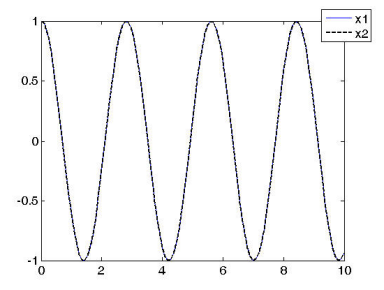
\includegraphics[width=0.5\linewidth]{fig_20_2}
		\label{fig:fig_20_2}
	\end{figure}
	\bigbreak
Because we have set the initial conditions consistent with one of the eigenvectors, the two masses oscillate in unison.
	\bigbreak
\item $x_{1}=1, x_{2}=-0.6$
	\bigbreak
\begin{lstlisting}[numbers=none]
>> tspan=[0,10];
>> y0=[1,-0.6,0,0];
>> [t,y]=ode45('dxdt',tspan,y0);
>> plot(t,y(:,1),t,y(:,2),'--')
>> legend('x1','x2')
\end{lstlisting}
	\bigbreak
	\begin{figure}[H]
		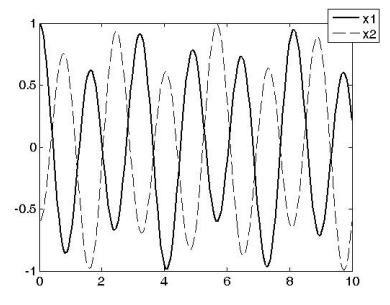
\includegraphics[width=0.5\linewidth]{fig_20_3}
		\label{fig:fig_20_3}
	\end{figure}
	\bigbreak
Now, because the initial conditions do not correspond to one of the eigenvectors, the motion involves the superposition of both modes.
	\bigbreak
\end{enumerate}



\section{}
\begin{lstlisting}[numbers=none]
function [e, v] = powmax(A)
%	 [e, v] = powmax(A):
%		 uses the power method to find the highest eigenvalue and
%		 the corresponding eigenvector
% input:
%	 A = matrix to be analyzed
% output:
%	 e = eigenvalue
%	 v = eigenvector
es = 0.0001;
maxit = 100;
n = size(A);
for i=1:n
	 v(i)=1;
end
v = v';
e = 1;
iter = 0;
while (1)
	 eold = e;
	 x = A*v;
	 [e,i] = max(abs(x));
	 e = sign(x(i))*e;
	 v = x/e;
	 iter = iter + 1;
	 ea = abs((e - eold)/e) * 100;
	 if ea <= es | iter >= maxit, break, end
end 
\end{lstlisting}
	\bigbreak
Application to solve Prob. \ref{sec:sec_20_2}
	\bigbreak
\begin{lstlisting}[numbers=none]
>> A = [2 2 10;8 3 4;10 4 5];
>> [e, v] = powmax(A)
e =
	 16.2741
v =
	 0.8113
	 0.7903
	 1.0000 
\end{lstlisting}
	\bigbreak



\section{}
\begin{lstlisting}[numbers=none]
function [e, v] = powmin(A)
%	 [e, v] = powmin(A):
%	 uses the power method to find the lowest eigenvalue and
%	 the corresponding eigenvector
% input:
%	 A = matrix to be analyzed
% output:
%	 e = eigenvalue
%	 v = eigenvector
es = 0.0001;
maxit = 100;
n = size(A);
for i=1:n
	 v(i)=1;
end
v = v';
e = 1;
Ai = inv(A);
iter = 0;
while (1)
	 eold = e;
	 x = Ai*v;
	 [e,i] = max(abs(x));
	 e = sign(x(i))*e;
	 v = x/e;
	 iter = iter + 1;
	 ea = abs((e - eold)/e) * 100;
	 if ea <= es | iter >= maxit, break, end
end
e = 1./e; 
\end{lstlisting}
	\bigbreak
Application to solve Prob. \ref{sec:sec_20_2}
	\bigbreak
\begin{lstlisting}[numbers=none]
>> [e, v] = powmin(A)
e =
	 -0.1815
v =
	 -0.3341
	 1.0000
	 -0.1271
\end{lstlisting}
\end{document}